
\documentclass[12pt]{article}
\usepackage{enumitem}
\usepackage{geometry}
\usepackage{graphicx}
\geometry{margin=1in}

\title{TestRail Report – Snapshot 3}
\author{Haonan Ma}
\date{\today}

\begin{document}

\maketitle

\section*{Overview}
This document contains the functional, performance, and security test cases implemented and verified during Snapshot 3 of the LAPD1 Transcript Analysis System project. The focus of this phase was on DOCX file format support, expanded NLP entity recognition, flag classification, export functionality, and performance handling of large transcripts.

\section*{Snapshot Summary Image}
\begin{center}
    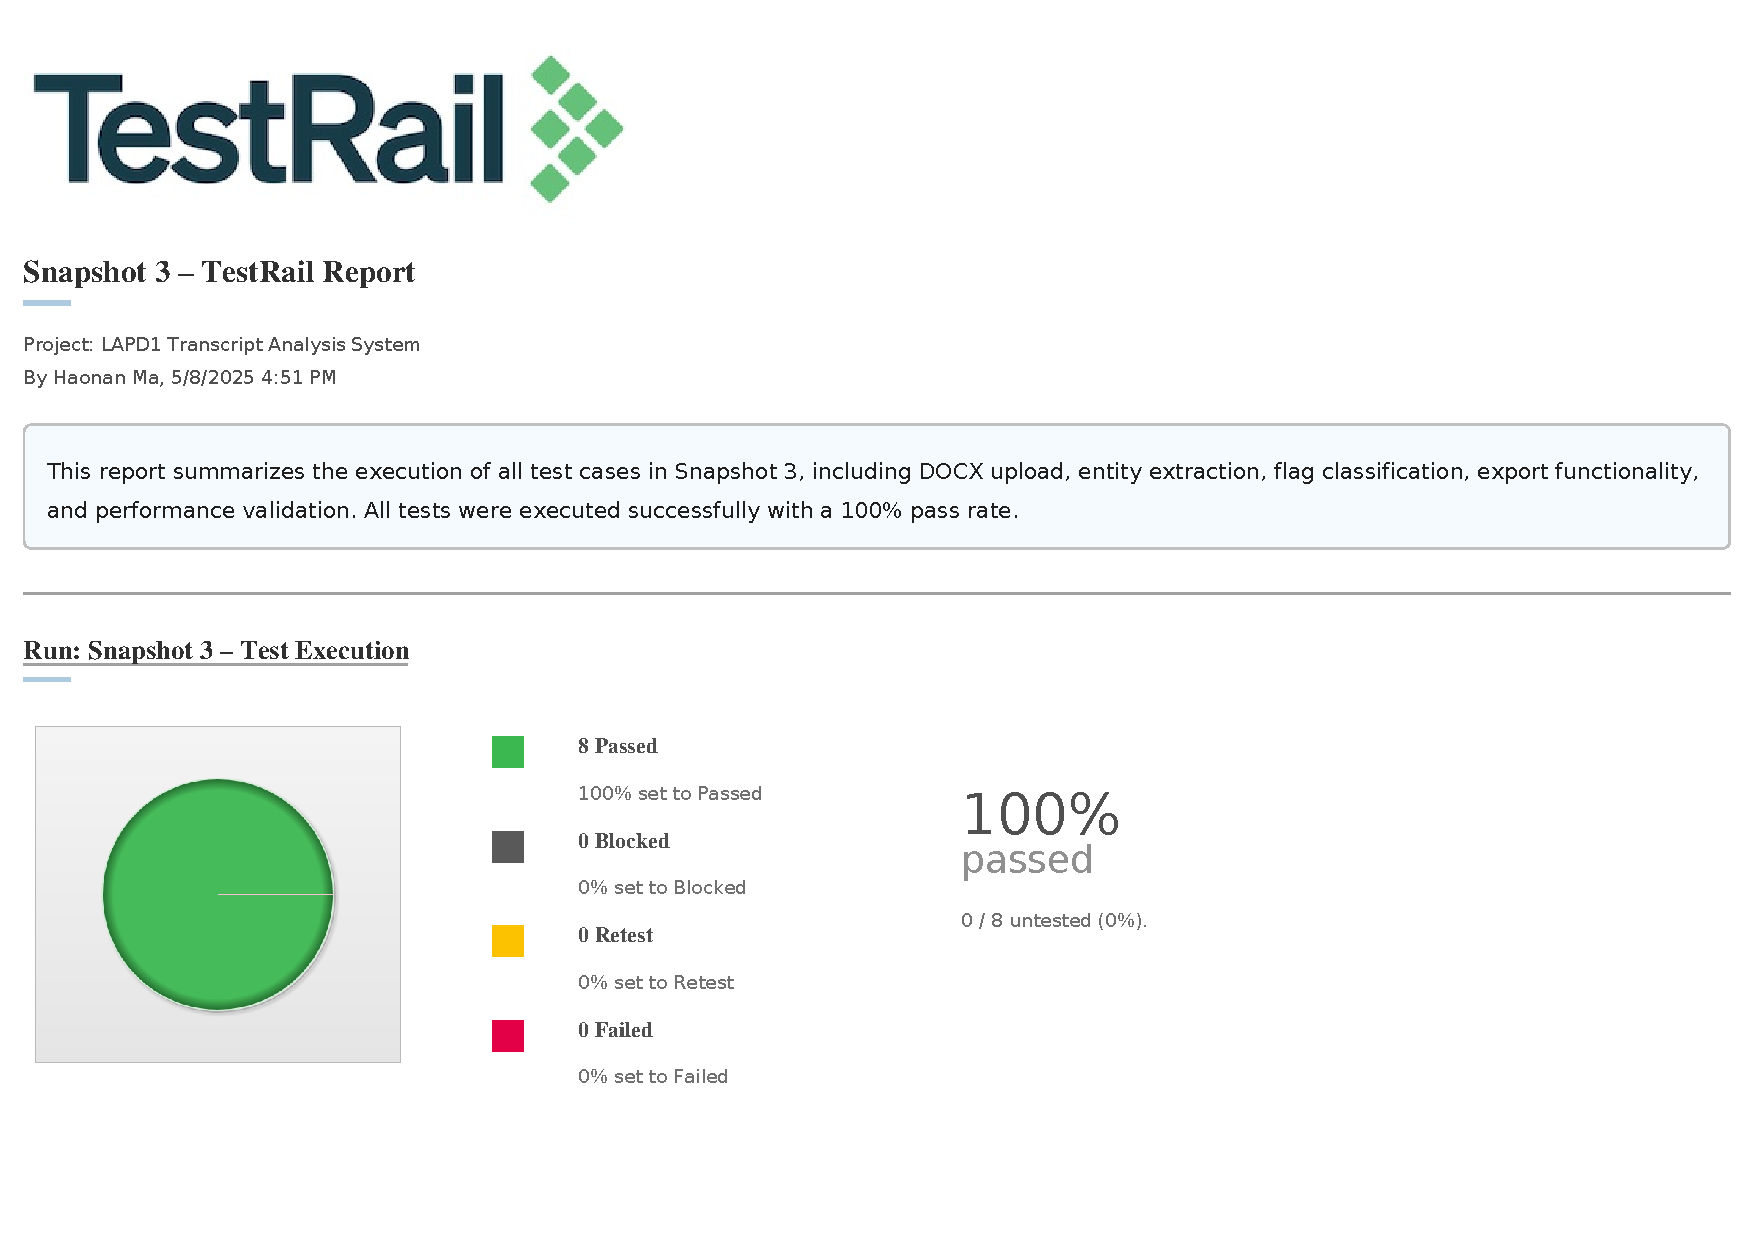
\includegraphics[width=\textwidth]{snapshot3image}
\end{center}

\section*{Test Cases}

\subsection*{Test Case 1: Upload DOCX File and Analyze}
\textbf{Type:} Functional \\
\textbf{Priority:} Medium \\
\textbf{Estimate:} 4m \\
\textbf{Preconditions:} User is logged in and on the upload page. \\
\textbf{Steps:}
\begin{enumerate}[label=\arabic*.]
\item Click the “Choose File” button.
\item Select a .docx transcript file from the local machine.
\item Click the “Analyze” button to initiate processing.
\end{enumerate}
\textbf{Expected Result:} The file is uploaded successfully and analyzed just like a PDF. Entity extraction and flagging proceed as expected.

\subsection*{Test Case 2: Extract Location Entity from Transcript}
\textbf{Type:} Functional \\
\textbf{Priority:} High \\
\textbf{Estimate:} 5m \\
\textbf{Preconditions:} A valid transcript with location-based information is available. \\
\textbf{Steps:}
\begin{enumerate}[label=\arabic*.]
\item Upload transcript containing named locations.
\item Click “Analyze”.
\item Review the extracted entity results.
\end{enumerate}
\textbf{Expected Result:} The system correctly identifies and labels locations as distinct entities.

\subsection*{Test Case 3: Detect Flag Category – Misconduct vs Inconsistency}
\textbf{Type:} Functional \\
\textbf{Priority:} High \\
\textbf{Estimate:} 6m \\
\textbf{Preconditions:} Transcript includes both misconduct and conflicting statements. \\
\textbf{Steps:}
\begin{enumerate}[label=\arabic*.]
\item Upload transcript with mixed flag types.
\item Run analysis.
\item Inspect categorized results.
\end{enumerate}
\textbf{Expected Result:} Flags are correctly categorized and displayed (e.g., “Misconduct”, “Inconsistency”).

\subsection*{Test Case 4: Export Entity-Flag Mapping to CSV}
\textbf{Type:} Functional \\
\textbf{Priority:} Medium \\
\textbf{Estimate:} 5m \\
\textbf{Preconditions:} Analyzed transcript is available with entities and flags. \\
\textbf{Steps:}
\begin{enumerate}[label=\arabic*.]
\item Open analysis result page.
\item Click “Export” and select CSV.
\item Open downloaded file.
\end{enumerate}
\textbf{Expected Result:} Exported CSV includes rows of entities and their related flags, formatted correctly.

\subsection*{Test Case 5: Analyze Long Transcript (>30 Pages)}
\textbf{Type:} Performance \\
\textbf{Priority:} Medium \\
\textbf{Estimate:} 8m \\
\textbf{Preconditions:} A 30+ page transcript is available. \\
\textbf{Steps:}
\begin{enumerate}[label=\arabic*.]
\item Upload the long transcript.
\item Click “Analyze”.
\item Monitor system performance.
\end{enumerate}
\textbf{Expected Result:} System completes analysis without crash or timeout within acceptable processing time.

\subsection*{Test Case 6: Block Upload of Encrypted Files}
\textbf{Type:} Security \\
\textbf{Priority:} High \\
\textbf{Estimate:} 3m \\
\textbf{Preconditions:} Encrypted (password-protected) document is ready. \\
\textbf{Steps:}
\begin{enumerate}[label=\arabic*.]
\item Attempt to upload encrypted file.
\item Observe system response.
\end{enumerate}
\textbf{Expected Result:} System blocks upload and displays a message: “Encrypted files are not supported.”

\subsection*{Test Case 7: Entity Filtering in Dashboard Search}
\textbf{Type:} Functional \\
\textbf{Priority:} Medium \\
\textbf{Estimate:} 4m \\
\textbf{Preconditions:} Several transcripts with various entity types have been uploaded. \\
\textbf{Steps:}
\begin{enumerate}[label=\arabic*.]
\item Go to dashboard search.
\item Apply entity type filter.
\item Search using keyword.
\end{enumerate}
\textbf{Expected Result:} Results list only includes transcripts matching the filter and query.

\subsection*{Test Case 8: Auto-Queue Analysis for Multiple Uploads}
\textbf{Type:} Functional \\
\textbf{Priority:} Medium \\
\textbf{Estimate:} 6m \\
\textbf{Preconditions:} At least 3 files ready for upload. \\
\textbf{Steps:}
\begin{enumerate}[label=\arabic*.]
\item Upload files back-to-back without waiting.
\item Wait for analysis to queue and complete.
\end{enumerate}
\textbf{Expected Result:} All files are processed sequentially without skipping or failure.

\end{document}
